% !TEX program = xelatex
% -*- coding:utf-8 -*-
\documentclass[12pt,aspectratio=169,mathserif]{beamer}
% 设置为 Beamer 文档类型，设置字体为 12pt，长宽比为16:9，数学字体为 serif 风格

%%%%-----导入宏包-----%%%%
\usepackage{zju}            % 导入 zju 模板宏包
\usepackage{amsmath,amsfonts,amssymb,bm}
\usepackage{color}
\usepackage{graphicx,hyperref,url}
\usepackage{metalogo}
\usepackage{fontspec}
\usepackage{xeCJK}
\usepackage{tcolorbox}
\usepackage{tikz}
\usetikzlibrary{arrows.meta,positioning,calc,fit}
\beamertemplateballitem

%%%%------------------------%%%%%
\catcode`\。=\active
\newcommand{。}{．}
%%%%%%%%%%%%%%%%%%%%%

%%%%----首页信息设置----%%%%
\title[基于增量奇异值分解的参数化PDE降阶方法研究]{基于增量奇异值分解的参数化PDE降阶方法研究}
\author[Zhouyue Qian]{钱周越 \\ 指导老师：李雨文}
\institute[ZJU]{数学科学学院 \\ 浙江大学}
\date[May 22, 2026]{2026年5月22日}

%%%%----自定义命令----%%%%
\newcommand{\R}{\mathbb{R}}
\newcommand{\norm}[1]{\left\lVert #1\right\rVert}
\newcommand{\ipW}[2]{\left\langle #1, #2\right\rangle_{W}}

\begin{document}

%========================================================
\begin{frame}
  \titlepage
\end{frame}

%========================================================
\section{目录}
\begin{frame}
  \frametitle{目录}
  \tableofcontents
\end{frame}

%========================================================
\section{研究背景与动机}

\begin{frame}
  \centering
  \Huge \insertsection
\end{frame}

%--------------------------------------------------------
\begin{frame}
\frametitle{参数化椭圆方程与many-query场景}

考虑含参数的一族椭圆型方程：
\[
-\nabla\cdot\big(a(x;\mu)\nabla u(x;\mu)\big)=f(x),\quad x\in\Omega,\ \mu\in\mathcal{P}\subset\R^p .
\]

有限元离散后得到大规模线性系统：
\[
A(\mu)u_h(\mu)=f(\mu),\quad A(\mu)\in\R^{N\times N},\ u_h(\mu)\in\R^{N},\ N\gg 1.
\]

\begin{itemize}
  \item 参数 $\mu$ 改变 $\Rightarrow$ 需反复求解不同的 $A(\mu)u=f$
  \item 高精度 FEM 解昂贵，重复求解成本不可接受
  \item \textbf{目标：} 在保证精度的前提下显著降低多参数重复求解开销
\end{itemize}

\end{frame}

%--------------------------------------------------------
\begin{frame}
\frametitle{缩减基方法（RB）：离线/在线分解}

核心思想：用低维子空间逼近高维有限元解
\[
u_h(\mu)\approx V_r a(\mu),\quad V_r\in\R^{N\times r},\ r\ll N .
\]

Galerkin 投影到 $V_r$：
\[
V_r^T A(\mu)V_r\, a(\mu)=V_r^T f(\mu),
\]
在线阶段仅需解 $r\times r$ 系统。

\begin{itemize}
  \item \textbf{离线阶段：} 构造缩减基 $V_r$（主要计算瓶颈）
  \item \textbf{在线阶段：} 快速求解并恢复 $u_r(\mu)=V_r a(\mu)$
\end{itemize}

\end{frame}

%--------------------------------------------------------
\begin{frame}
\frametitle{POD/SVD：最优低秩子空间与“快照矩阵”}

收集 $m$ 个参数样本对应的 FEM 快照：
\[
U=[u_h(\mu_1),\dots,u_h(\mu_m)]\in\R^{N\times m}.
\]

做 SVD（或加权 core SVD）得到 POD 基：
\[
U=\Phi\Sigma\Psi^T,\quad V_r:=\Phi_{(:,1:r)}.
\]

截断误差（Frobenius 范数意义下的最优性）：
\[
\|U-U_r\|_F^2=\sum_{i>r}\sigma_i^2,\quad U_r=\Phi_r\Sigma_r\Psi_r^T.
\]

\textbf{批处理 SVD 的三大瓶颈：}
\begin{enumerate}
  \item 计算复杂度 $\mathcal{O}(Nm^2)$
  \item 内存峰值 $\mathcal{O}(Nm)$
  \item 无法流式处理
\end{enumerate}

\end{frame}

%========================================================
\section{经典增量SVD及其正交性问题}

\begin{frame}
  \centering
  \Huge \insertsection
\end{frame}

%--------------------------------------------------------
\begin{frame}
\frametitle{加权 Core SVD 框架}

由于快照来自有限元离散，自然内积为加权形式（质量矩阵 $W=M$）：
\[
\langle u,v\rangle_W = u^{\mathrm{T}}Wv.
\]

Core SVD 分解：
\[
U = Q\Sigma R^{\mathrm{T}},\quad Q^{\mathrm{T}}WQ = I,\quad R^{\mathrm{T}}R = I,
\]
其中 $\Sigma = \mathrm{diag}(\sigma_1, \ldots , \sigma_r)$，$\sigma_1 \geq \dots \geq \sigma_r > 0$。

\end{frame}

%--------------------------------------------------------
\begin{frame}
\frametitle{Brand 经典增量 SVD 算法}

已知 $U_{\ell}=Q\Sigma R^{\mathrm{T}}$（rank-$k$ core SVD），新快照 $u_{\ell+1}$：

\begin{enumerate}
  \item 投影与加权残差：
  \[
  d=Q^{\mathrm{T}}(W u_{\ell+1}),\quad e=u_{\ell+1}-Q d,\quad p=\sqrt{e^{\mathrm{T}}W e}.
  \]
  \item 构造小矩阵 $Y=\begin{bmatrix}\Sigma & d\\0 & p\end{bmatrix}\in\mathbb{R}^{(k+1)\times(k+1)}$，计算 SVD：$Y=Q_Y\Sigma_Y R_Y^T$。
  \item 更新分解：
  \[
  Q \leftarrow [Q\mid \tilde{e}] Q_Y,\quad \Sigma \leftarrow \Sigma_Y,\quad R \leftarrow \begin{bmatrix} R & 0\\0 & 1 \end{bmatrix} R_Y.
  \]
\end{enumerate}

\textbf{优势：} 单步复杂度 $\mathcal{O}(k^3)$，远低于重算全矩阵。

\end{frame}

%--------------------------------------------------------
\begin{frame}
\frametitle{经典算法的正交性退化问题}

Brand 算法中 $Q \leftarrow [Q \mid \tilde{e}] Q_Y$ 涉及小正交矩阵 $Q_Y$ 的连乘：
\[
Q \leftarrow Q \prod Q_Y^{(i)}.
\]

在有限精度下，连乘累积舍入误差导致 $Q^T W Q$ 严重偏离单位矩阵。

\begin{block}{Brand (2006) 指出的开放问题}
\textit{“为了保证一定的整体数值精度水平，需要多久进行一次重正交化是一个开放问题；这不会改变整体复杂度。”}
\end{block}

传统重正交化计算开销巨大，尤其在加权内积下。

\end{frame}

%========================================================
\section{改进算法原理}

\begin{frame}
  \centering
  \Huge \insertsection
\end{frame}

%--------------------------------------------------------
\begin{frame}
\frametitle{Zhang (2022) 改进算法的核心思想}

通过\textbf{累积更新策略}，将 $s$ 步更新凝聚为一次对扩展矩阵的 SVD，\textbf{彻底避免小正交矩阵连乘}。

\vspace{0.3cm}
\textbf{定理（累积更新）：} 设 $Q\Sigma R^{\mathrm{T}}$ 为 $U_\ell$ 的 rank-$k$ core SVD，$s$ 个连续新快照的加权残差均为零。构造
\[
M_s = \bigl[\Sigma \mid Q^{\mathrm{T}}W u_{\ell+1}\mid \cdots \mid Q^{\mathrm{T}}W u_{\ell+s}\bigr]\in\mathbb{R}^{k\times(k+s)},
\]
并令 $M_s = \widehat{Q}\widehat{\Sigma}\widehat{R}^{\mathrm{T}}$ 为其薄 SVD。则一步更新
\[
Q\leftarrow Q\widehat{Q},\quad \Sigma \leftarrow \widehat{\Sigma},\quad R\leftarrow \begin{bmatrix} R & 0 \\ 0 & I_s \end{bmatrix}\widehat{R}
\]
与逐次应用 Brand 更新完全等价，且 $\widehat{Q},\widehat{R}$ 数值正交。

\end{frame}

%--------------------------------------------------------
\begin{frame}
\frametitle{算法优势与复杂度对比}

\begin{table}[h]
\centering
\caption{不同构基方法的复杂度和内存对比}
\begin{tabular}{lccc}
\hline
方法 & 时间复杂度 & 峰值内存 & 流式处理 \\
\hline
Batch SVD & $\mathcal{O}(N n^2)$ & $\mathcal{O}(N n)$ & 否 \\
Brand ISVD (经典) & $\mathcal{O}(N n r)$ & $\mathcal{O}((N+n)r)$ & 是 \\
Zhang ISVD (改进) & $\mathcal{O}(N n r)$ & $\mathcal{O}((N+n)r)$ & 是 \\
\hline
\end{tabular}
\end{table}

\begin{itemize}
  \item \textbf{数值稳定性：} 从根源上消除了正交性退化，无需重正交化
  \item \textbf{内存效率：} 与总样本数 $n$ 解耦，支持流式处理
  \item \textbf{计算效率：} 常数因子显著降低
\end{itemize}

\end{frame}

%========================================================
\section{数值实验}

\begin{frame}
  \centering
  \Huge \insertsection
\end{frame}

%--------------------------------------------------------
\begin{frame}
\frametitle{实验设置}

三个层次的数值实验：

\begin{enumerate}
  \item \textbf{算法基准测试：} 流式矩阵更新，验证正交性保持与分解正确性
  \item \textbf{1D 参数化 PDE：} 对比批次 SVD、经典 Brand ISVD 和 Zhang ISVD
  \item \textbf{2D 大规模 PDE：} 两个/三个参数模型，测量内存压缩比、离线时间加速比和降阶精度
\end{enumerate}

加权内积矩阵 $W$ 取为质量矩阵 $M$，有限元框架实现。

\end{frame}

%--------------------------------------------------------
% 新增：统一罗列参数化 PDE 模型
\begin{frame}
\frametitle{参数化 PDE 模型}

\textbf{1D 变系数椭圆方程：}
\[
-\frac{d}{dx}\bigl((1+\mu x)\frac{du}{dx}\bigr)=1,\quad x\in(0,1),\ u(0)=u(1)=0,
\]
参数 $\mu\in[0,1]$，等距取 200 个训练参数、100 个测试参数。有限元离散单元数 $N=500$。

\vspace{0.3cm}
\textbf{2D 椭圆方程（两个参数）：}
\[
-\nabla\cdot\bigl((1+\mu_1 x + \mu_2 y)\nabla u\bigr)=1,\quad (x,y)\in(0,1)^2,
\]
齐次 Dirichlet 边界条件。$40\times40$ 网格，$N=1600$，参数 $\mu_1,\mu_2\in[-0.2,0.2]$。

\vspace{0.3cm}
\textbf{2D 椭圆方程（三个参数）：}
\[
-\nabla\cdot\bigl((1+\mu_1 x + \mu_2 y + \mu_3 xy)\nabla u\bigr)=1,\quad (x,y)\in(0,1)^2,
\]

\end{frame}

%--------------------------------------------------------
\begin{frame}
\frametitle{更新后的ISVD算法正交性演化对比（基准测试）}

\begin{columns}
\column{0.5\textwidth}
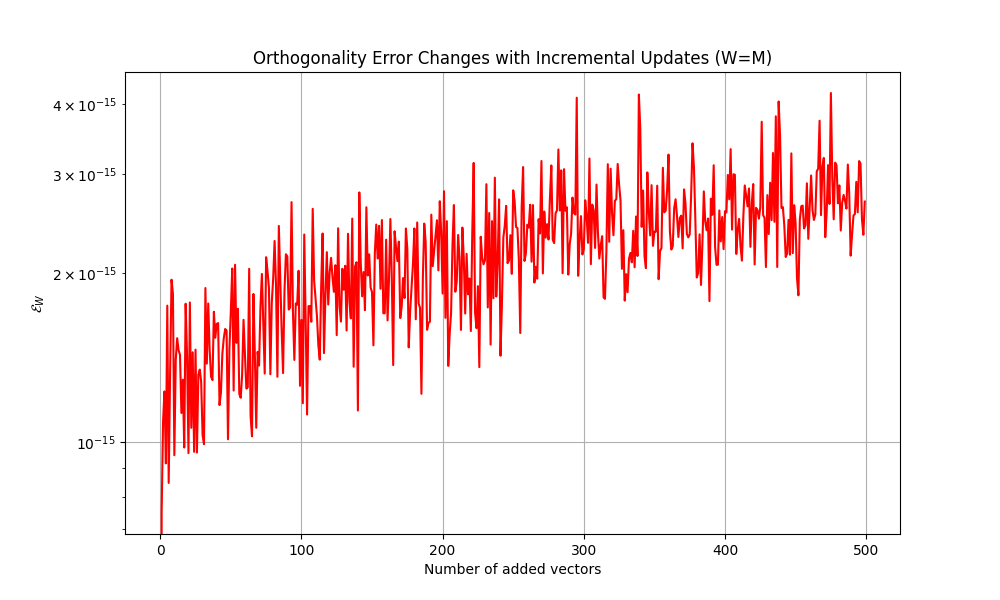
\includegraphics[width=\textwidth]{figure/simple_orthogonality_error.png}
\column{0.5\textwidth}

\vspace{0.2cm}
\textbf{结论：} Brand 算法在 400 次更新后正交性急剧恶化；Zhang 改进算法始终保持在 $10^{-14}$ 以下。
\end{columns}

\end{frame}

%--------------------------------------------------------
\begin{frame}
\frametitle{1D 参数化 PDE：离线构基时间对比}

\begin{columns}
\column{0.5\textwidth}
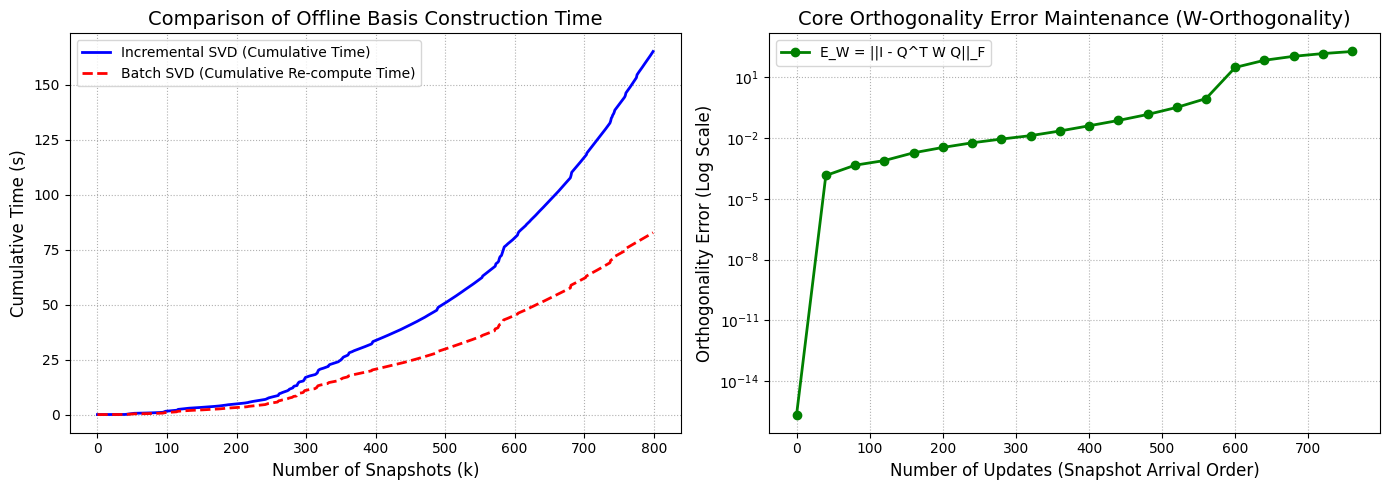
\includegraphics[width=\textwidth]{figure/1D.png}
\column{0.5\textwidth}
\begin{itemize}
  \item 批次 SVD 累计时间呈二次增长
  \item 经典 Brand ISVD 因正交性退化，后期时间急剧增加
  \item 400 步后 Brand 正交性误差 $\mathcal{E}_W(Q)$ 升至 $10^1$，导致数值不稳定
\end{itemize}
\end{columns}

\end{frame}

%--------------------------------------------------------
\begin{frame}
\frametitle{1D 参数化 PDE：Zhang ISVD 正交性}

\begin{columns}
\column{0.5\textwidth}
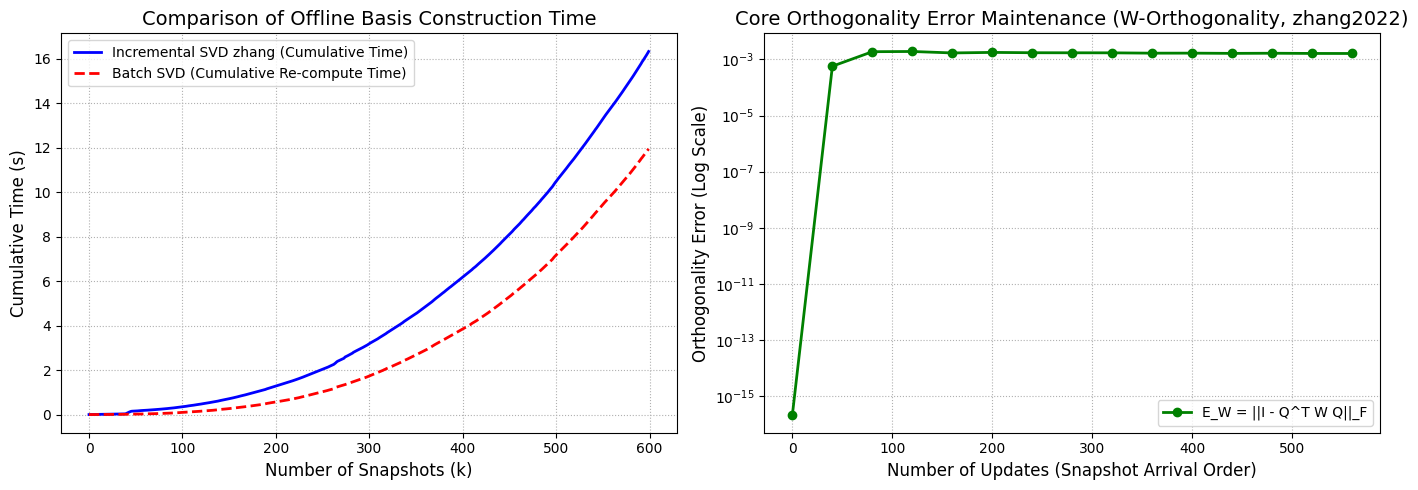
\includegraphics[width=\textwidth]{figure/1D_zhang.png}
\column{0.5\textwidth}
加权正交性误差：
\[
\mathcal{E}_W(Q) = \| I - Q^T W Q \|_F
\]
其中 $\|\cdot\|_F$ 为 Frobenius 范数，$W$ 为质量矩阵。
\begin{itemize}
  \item Zhang ISVD 在整个 550 次更新中 $\mathcal{E}_W(Q)$ 始终 $<10^{-3}$
  \item 远优于经典 Brand 在 400 步后的完全发散
\end{itemize}
\end{columns}

\end{frame}

%--------------------------------------------------------
\begin{frame}
\frametitle{1D 参数化 PDE：单步时间差分析}

\begin{columns}
\column{0.5\textwidth}
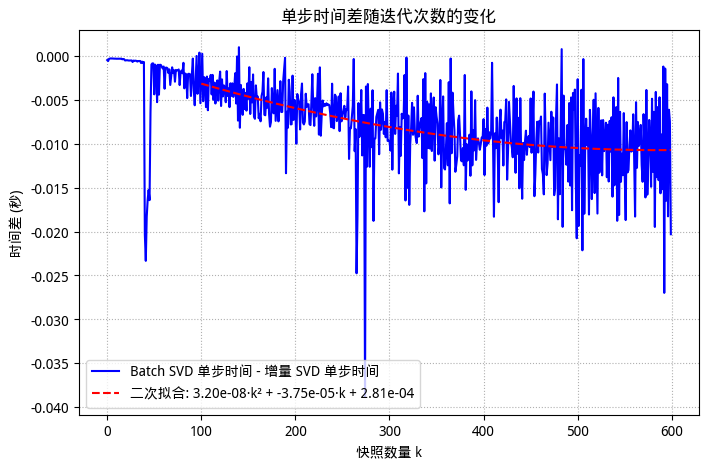
\includegraphics[width=\textwidth]{figure/1D_zhang_time.png}
\column{0.5\textwidth}
拟合曲线：
\[
3.20\times10^{-8}k^2 - 3.75\times10^{-5}k + 2.81\times10^{-4}
\]
在 1D 问题中，实验中ISVD用时呈二次增长，参数空间维数较低，增量 SVD 的效率优势不明显。因此在 2D 实验中，我们将参数维数增至 2~3，总快照数提升至 50,000，以更充分地展示改进算法的性能。

\end{columns}

\end{frame}

%--------------------------------------------------------
\begin{frame}
\frametitle{2D 大规模 PDE（两个参数）}

\centering
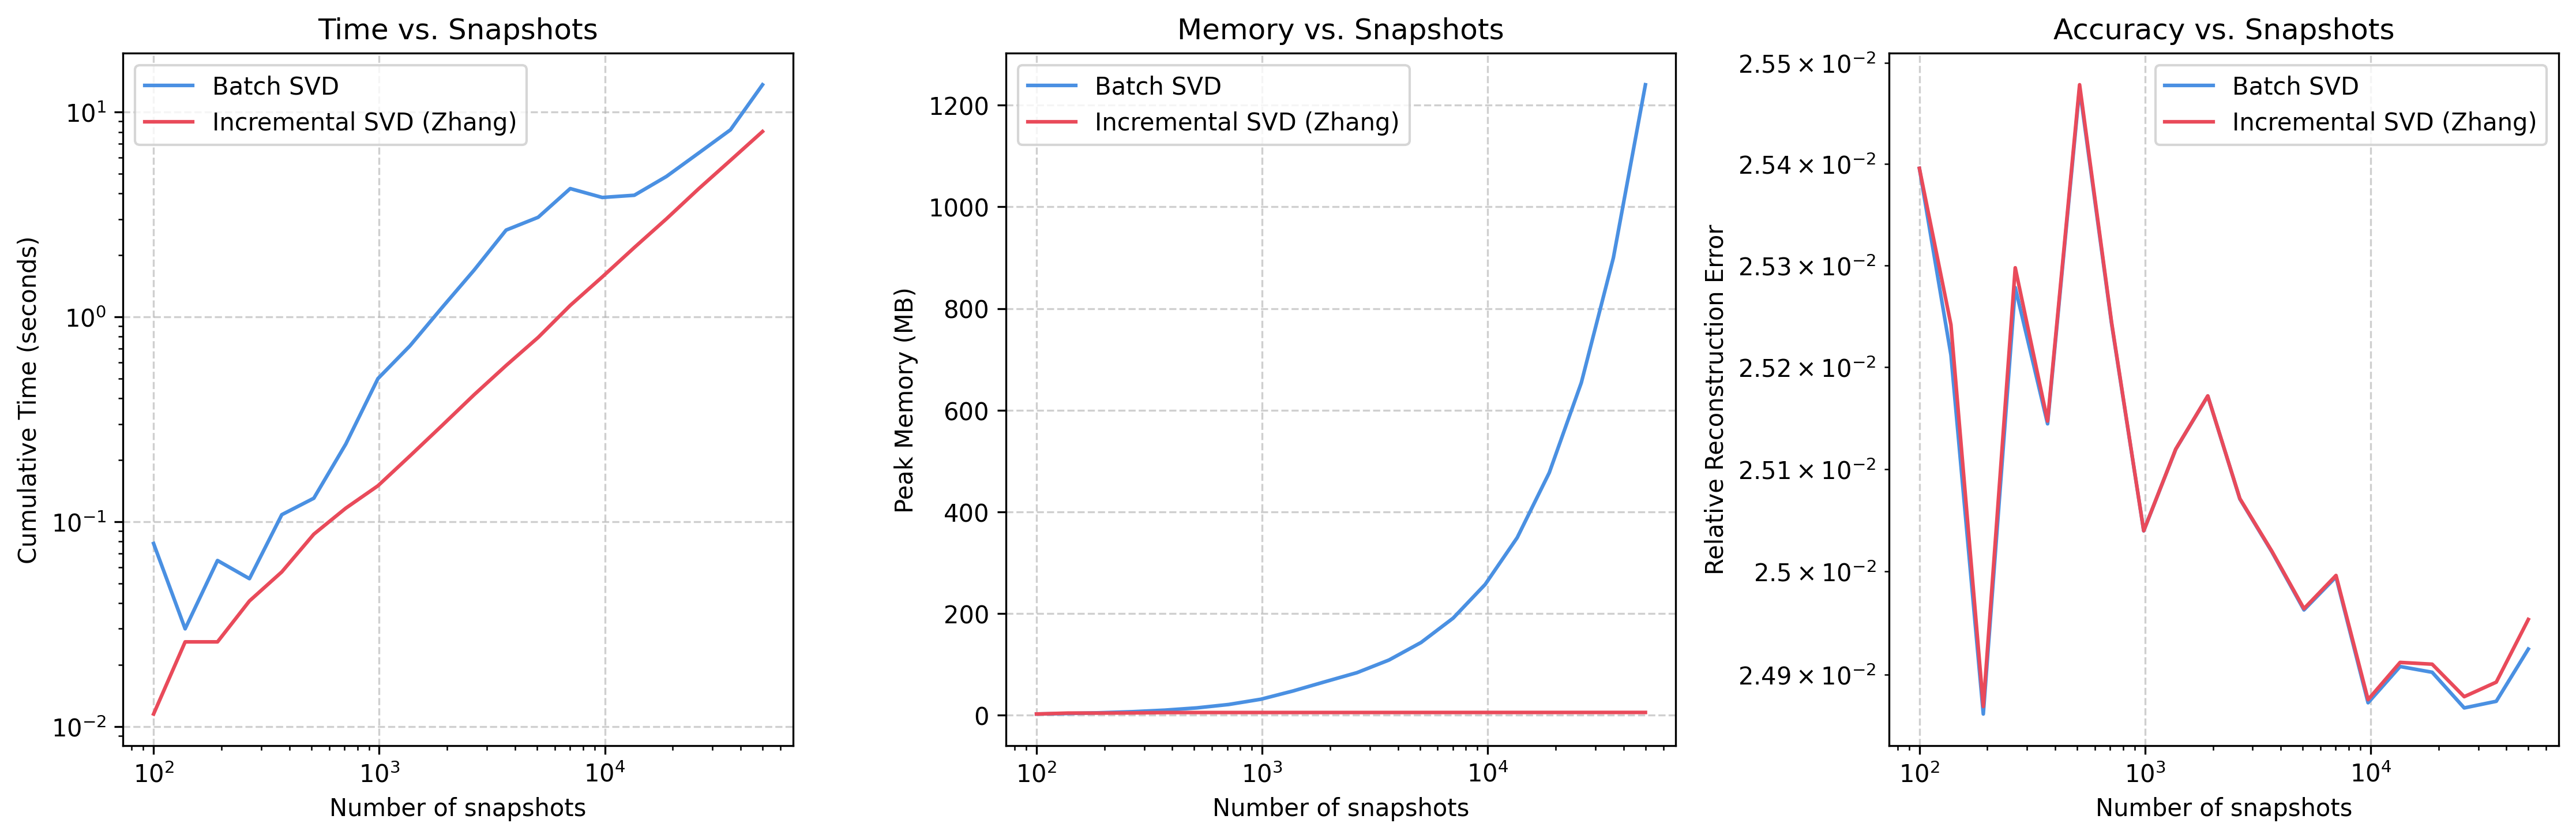
\includegraphics[width=0.7\textwidth]{figure/svd_vs_snapshots_adaptive_r.png}

\begin{table}[h]
\centering
\begin{tabular}{|l|c|c|}
\hline
指标 & Batch SVD & Zhang ISVD \\
\hline
峰值内存 & 1240 MB & $\sim$10 MB \\
压缩比 & 1× & 120× \\
累计时间 & 较高 & $\sim$8秒（近似线性） \\
重建误差 & $10^{-2}$ 量级 & $10^{-2}$ 量级 \\
\hline
\end{tabular}
\end{table}

\end{frame}

%--------------------------------------------------------
\begin{frame}
\frametitle{2D 大规模 PDE（三个参数）}

\centering

\includegraphics[width=0.7\textwidth]{figure/svd_vs_snapshots.png}

\begin{table}[h]
\centering
\begin{tabular}{|l|c|c|}
\hline
指标 & Batch SVD & Zhang ISVD \\
\hline
峰值内存 & 1240.3 MB & 10.3 MB \\
压缩比 & 1× & 120× \\
累计时间 & 12.39 s & 8.43 s \\
最终重建误差 & $2.1\times10^{-7}$ & $1.5\times10^{-5}$ \\
\hline
\end{tabular}
\end{table}

\end{frame}

%--------------------------------------------------------
\begin{frame}
\frametitle{精度与稳定性讨论}

\begin{itemize}
  \item \textbf{正交性：} Zhang 改进 ISVD 加权正交性误差始终 $<10^{-14}$（基准测试）或 $<10^{-3}$（1D PDE），远优于经典 Brand 的发散。
  \item \textbf{内存：} 峰值内存压缩 120 倍，存储节约率 $>99\%$。
  \item \textbf{时间：} 累计时间加速比约 1.47 倍，且呈近似线性增长。
  \item \textbf{精度：} 重建误差 $1.5\times10^{-5}$ vs. 批次 $2.1\times10^{-7}$，初始误差短暂上升后迅速收敛。
\end{itemize}

\textbf{结论：} 改进 ISVD 在内存、时间、精度之间找到了实用的平衡点，特别适合大规模 many-query 场景。

\end{frame}

%========================================================
\section{结论与展望}

\begin{frame}
  \centering
  \Huge \insertsection
\end{frame}

%--------------------------------------------------------
\begin{frame}
\frametitle{结论}

\begin{enumerate}
  \item 完整复现了加权 core SVD 框架与 Brand 经典增量算法，揭示了正交性退化的根源。
  \item 实现了 Zhang (2022) 改进算法，通过累积更新策略从根本上避免小正交矩阵连乘。
  \item 数值实验表明：
    \begin{itemize}
      \item 改进 ISVD 能够长期保持加权正交性
      \item 峰值内存压缩一个数量级以上（最高 120 倍）
      \item 离线时间显著缩短（加速比达 1.47 倍）
      \item 逼近精度与批次 POD 相当
    \end{itemize}
  \item 为大规模参数化 PDE 的高效降阶提供了兼具数值稳定性与计算效率的可行方案。
\end{enumerate}

\end{frame}

%--------------------------------------------------------
\begin{frame}
\frametitle{未来展望}

\begin{itemize}
  \item \textbf{理论分析：} 建立累积更新策略的误差上界，量化块大小与截断阈值的影响。
  \item \textbf{超大规模扩展：} 验证在三维非定常流动（$N>10^5$，$n>10^6$）中的可扩展性。
  \item \textbf{自适应策略：} 根据残差范数动态调整更新频率，根据奇异值谱自动选择截断精度。
  \item \textbf{完全在线离线构基：} 与贪婪采样、后验误差估计器深度集成，实现边采样边构基。
\end{itemize}

\end{frame}

%========================================================
\section{参考文献}

\begin{frame}{参考文献}
\footnotesize
\begin{thebibliography}{99}

\bibitem{hesthaven2015}
J. S. Hesthaven, G. Rozza, B. Stamm,
\emph{Certified Reduced Basis Methods for Parametrized Partial Differential Equations},
Springer, 2015.

\bibitem{patera_rozza}
A. T. Patera, G. Rozza,
\emph{Reduced Basis Approximation and A Posteriori Error Estimation for Parametrized PDEs},
MIT Pappalardo Graduate Monographs, 2007.

\bibitem{fareed2018}
H. Fareed, J. R. Singler, Y. Zhang,
Incremental proper orthogonal decomposition for PDE simulation data,
\emph{Computers \& Mathematics with Applications}, 75(6):1942-1960, 2018.

\bibitem{brand2002}
M. Brand,
Incremental singular value decomposition of uncertain data with missing values,
\emph{ECCV}, 2002.

\bibitem{brand2006}
M. Brand,
Fast low-rank modifications of the thin singular value decomposition,
\emph{Linear Algebra and its Applications}, 415(1):20-30, 2006.

\bibitem{zhang2022}
Y. Zhang,
An answer to an open question in the incremental SVD,
\emph{Numerical Linear Algebra with Applications}, 29(6):e2448, 2022.

\bibitem{golub2013matrix}
G. H. Golub, C. F. Van Loan,
\emph{Matrix Computations}, 4th ed., Johns Hopkins University Press, 2013.

\end{thebibliography}
\end{frame}

%========================================================
\end{document}